\section{Converting Code Program Graph}
This section will briefly cover how the program graph is created.
Creating a program graph from the code (also called the program), is already a proven concept, therefore this paper will not delve into the details, but rather simply inform the reader.
The book used to show that the concept of creating a program graph from code is a proven concept is \cite{nielson_formal_2019}, specifically chapter 2.2.
A program graph consists of a finite set of nodes, an initial node and final node, a set of actions, and a finite set of edges.

These edges are directed and represent the flow of the program, and the nodes represent the state of the program. The actions are the atomic operations that the program can perform. The initial node is the starting point of the program, and the final node is the end of the program.

The program graph is created by parsing the code and creating nodes and edges that represent the flow of the code. For example, if the code is only an assignment, there will be a node for the initial state, a node for the final state, and an edge between them that represents the assignment. This is written as the following equation:
$edges(q_{\circ} \rightsquigarrow q_{\bullet})\llbracket x:=a \rrbracket = \{(q_{\circ}, x:=a, q_{\bullet})\}$
Where $q_{\circ}$ is the initial node, $q_{\bullet}$ is the final node, and $x:=a$ is the assignment. This then creates a set, that represents the program graph, that can be seen in \autoref{fig:tikz-program-graph-assignment}. This is a simple example, and the program graph can be more complex depending on the code, but the concept is the same.
Further examples can be found in \cite{nielson_formal_2019} Figure 2.6.

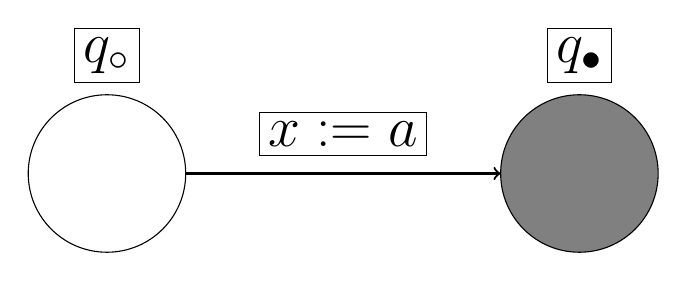
\begin{tikzpicture}
    \filldraw[fill=white, draw=black] (2,2) circle (1cm);
    \filldraw[fill=gray, draw=black] (8,2) circle (1cm);
    \node [draw] at (2,3.5) {\huge $q_{\circ}$};
    \node [draw] at (8,3.5) {\huge $q_{\bullet}$};
    \node [draw] at (5, 2.5) {\huge $x:=a$};
    \draw [thick, ->](3, 2) -- (7, 2);
\end{tikzpicture}